
\chapter{Przegląd badań - stan wiedzy}

\section{Podobieństwo szeregów czasowych - przegląd algorytmów}
\subsection{Landmark similarity}
Założenia: Ludzie uważają dwa wykresy za podobne, jeżeli ich punkty zwrotne są podobne, a reszta wykresu to krzywe łączące te punkty
\newline
Metoda zakłada zidentyfikowanie cech, które pozostają niezmienne po wykonaniu następujących transformacji
\begin{enumerate}
    \item Przesunięcie (Shifting) 
    \item Jednolite Skalowanie Amplitudy (Uniform Amplitude Scaling)
    \item Jednolite Skalowanie Czasu (Uniform Time Scaling)
    \item Jednolite Bi-skalowanie (Uniform Bi-scaling)
    \item Dopasowanie Czasu (Time Warping)
    \item Niejednolite Skalowanie Amplitudy (Non-uniform amplitude scaling)
\end{enumerate}
\begin{figure}[H]
    \centering
    \captionsetup{justification=centering,margin=0.5cm}
    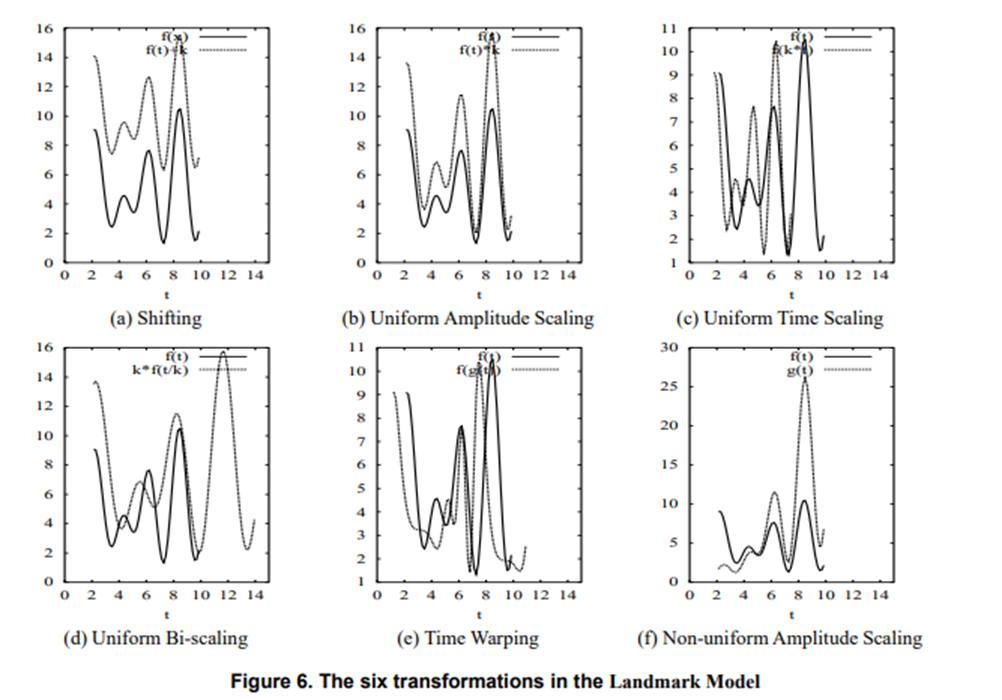
\includegraphics[scale=0.4]{figures/03-teoria/theSixTransformationsInTheLandmarkModel.png}
    \caption{Transformations in Landmark Model}
    \label{fig:scr46}
\end{figure}
\par
Wybór cech charakterystycznych:
Różne cechy są wykorzystywane do różnych zastosowań, od prostych cech (minima lokalne, maksima lokalne, punkty przełamania) do bardziej skomplikowanych
Im więcej typów cech, tym dokładniejsze wyniki
Punkt charakterystyczny n-tego rzędu danej krzywej jest wtedy, gdy pochodna n-tego rzędu znajduje się na tym punkcie – lokalne minima/maksima są punktami 1 rzędu, a punkty przegięcia – 2 rzędu
Im bardziej zmienny wykres, tym mniejsze znaczenie mają punkty charakterystyczne wyższych rzędów
\par
Wygładzanie: Minimal Distance/Percentage Principle (MDPP) 
Przykład MDPP(5, 5\%) – znaczy: pomiar raz na 5 dni, od 5\% wzrost lub spadek zaczyna być znaczący. Zmiany większe niż 5\% nie zostaną wygładzone
\par 
Obliczanie podobieństwa: Porównujemy sekwencje landmarków (a nie surowych danych)
\begin{itemize}
    \item Pomiar niezgodności (dissimilarity measurement)
    \item Pomiar zgodności (z wykorzystaniem MDPP)
\end{itemize}

\subsection{Dynamic Time Warping}
Metoda zakłada znalezienie optymalnego dopasowania punktów jednego przebiegu do drugiego, który ma najmniejszy koszt i spełnia wszystkie z poniższych warunków:
Założenia przy porównywaniu dwóch sekwencji:
\begin{itemize}
    \item Pierwsze oraz ostatnie punkty przebiegów są dopasowane do siebie
    \item Przebieg nie cofa się w czasie podczas dopasowywania
    \item Podczas dopasowania nie można wykonać zbyt długich kroków
    \item Koszt dopasowania jest sumą lokalnych odległości na tej ścieżce
\end{itemize}
Charakterystyka algorytmu:
\begin{itemize}
    \item Radzi sobie ze skalowaniem czasu 
    \item Radzi sobie z przesunięciem czasu
    \item Bardziej zwraca uwagę na konkretne wartości, w porównaniu do Landmark Similarity, który głównie zwraca uwagę na punkty zwrotne
\end{itemize}

\subsection{Longest Common Subsequence}
Jeżeli S1 i S2 to dwa ciągi, to Z jest ich wspólnym podciągiem jeżeli jest podciągiem zarówno S1, jak i S2
Dwa ciągi są podobne jeżeli:
(2 * Długość Z )/(Długość S1 + Długość S2) $>$= wybrana wartość progowa 

\subsection{Odległość Euklidesowa}
 Długość odcinka między punktami
\begin{itemize}
    \item Podatny na wartości odstające
    \item Nie radzi sobie ze zeskalowanymi wykresami
    \item Wykresy muszą być tej samej długości
    \item TODO:poszukać wariacje odległości Euklidesowej
\end{itemize}

\section{Metody normalizacji danych}

W pracach zajmujących się uczeniem maszynowym bardzo często występuje normalizacja danych. Przykładowo \cite{RuntimeEstimationALICE} wykorzystuje normalizacje Z-score, a w pracy \cite{BigDataParallelism} twórcy użyli skalowania Min-Max. Wykonuję się ją na etapie przygotowywania danych (ang. Preprocessing) najczęściej w celu poprawienia wyników algorytmów lub czasem nawet algorytmy wymagają znormalizowanych danych dla poprawnego działania \cite{standarization_effects}. Dzięki temu procesowi otrzymujemy wartości, które w zbiorze danych będą miały podobną skale.  W tej sekcji opisane zostaną popularne metody normalizacji danych, czyli \textbf{Min-Max} oraz \textbf{Z-score}. Jedna z tych metod zostanie użyta na danych wykorzystywanych w tej pracy.

\subsection{Min-Max}
Technika normalizacji Min-Max polega na odjęciu od wartości najmniejszej wartości z dziedziny i następnie podzielenie jej przez największą wartość z tej samej dziedziny. Tą metodę można przedstawić za pomocą następującego wzoru: 
\begin{equation}
\label{eqn:minmax}
A'_i = \frac{A_i-min(A)}{max(A) - min(A)}
\end{equation}
W ten sposób uzyskujemy przeskalowane wartości z zakresu od 0 do 1. Jest to dobra technika, jeżeli nie znamy rozkładu wartości naszych danych lub jeżeli wiemy, że nie jest to rozkład standardowy.

\subsection{Z-score}
Ten sposób normalizacji to skalowanie poprzez odjęcie od wartości średniej wszystkich wartości i następnie podzielenia przez odchylenie standardowe zbioru. Wzór prezentuje się następująco:
\begin{equation}
\label{eqn:minmax}
A'_i = \frac{A_i-mean(A)}{std(A)}
\end{equation}
Ta technika nie jest ograniczona przez żaden predefiniowany zakres wartości. Sprawia ona że średnia jest równa 0, a odchylenie standardowe 1. Użycie tej metody jest preferowane, jeżeli znamy rozkład wartości i jest on rozkładem standardowym.